\documentclass{beamer}

\usepackage{ucs}
\usepackage{amsfonts,amsmath}
\usepackage{stmaryrd}
\usepackage[utf8x]{inputenc}
\usepackage[protrusion=true,expansion=true]{microtype}
\usepackage{setspace}
\usepackage{graphicx}
\usepackage{natbib}
\usepackage{listings}
\usepackage{tikz}

\usepackage{../../macros}

\usetikzlibrary{automata, positioning, shapes.misc, chains}

\tikzset{
  state/.style={
    rounded rectangle,
    very thick,draw=black!50,
    top color=white, bottom color=black!20,
    minimum size=2em,
    text height=1.5ex,text depth=.25ex
  }
}

\date{\small January 28,\\[0.5em] \sf TLDI 2012}

\title{Safe incremental type-checking}

\author[Matthias Puech \& Yann Régis-Gianas] {
  Matthias Puech\inst{1,2} \and Yann Régis-Gianas\inst{2}
}

\institute {
  \inst 1 {Dept. of Computer Science, University of Bologna} \and
  \inst 2 {Univ. Paris Diderot, Sorbonne Paris Cité, PPS, CNRS,  ${\pi}r^2$, INRIA}
}

\setbeamertemplate{footline}[frame number]
\setbeamertemplate{navigation symbols}{}
\setbeamertemplate{itemize item}[circle]

\usefonttheme{serif}
\usecolortheme[rgb={0.7,0.2,0.2}]{structure}
\definecolor{greenish}{rgb}{0.20,0.48,0.09} % vert des exemples

\lstset{
  language=[Objective]Caml,
  basicstyle=\sf,
  columns=flexible,
  literate={->}{{$\to$ }}1 {*}{$\times$ }1 {>=}{{$\geq$}}1
  {<>}{{$\neq$}}1 {'a}{{$\alpha$}}1 {'b}{{$\beta$}}1 {'c}{{$\gamma$}}1
}

\begin{document}

\frame\titlepage

\section{Motivation}

\subsection{Type-checking}

\begin{frame}{\textcolor{gray}{Safe incremental} type-checking}

  \begin{block}{
      \only<1>{Weakly-typed programs need testing}
      \only<2->{Strongly-typed programs need less testing}
    }
    \vspace{1em}
    \begin{overlayarea}{\textwidth}{8em}
      \centering
      \only<1>{
        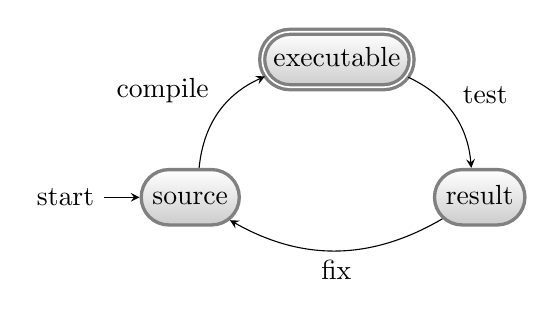
\begin{tikzpicture}[node distance=4em, auto, bend left, >=stealth]
          \node[initial, state] (source) {source};
          \node[accepting, state] (exec) [above right=of source] {executable};
          \node[state] (result) [below right=of exec] {result};

          \path[->]
          (source) edge node {compile} (exec)
          (exec) edge node {test} (result)
          (result) edge node {fix} (source) ;
        \end{tikzpicture}
      }

      \only<2->{
        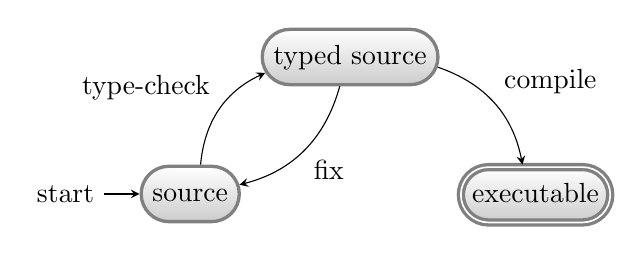
\begin{tikzpicture}[node distance=4em, auto, bend left, >=stealth]
          \node[initial, state] (source) {source};
          \node[state] (bool) [above right=of source] {typed source};
          \node[accepting, state] (exec) [below right=of bool] {executable};

          \path[->]
          (source) edge [bend left] node {type-check} (bool)
          (bool) edge [bend left] node {compile} (exec)
          (bool) edge [bend left] node {fix} (source);
        \end{tikzpicture}
      }
    \end{overlayarea}

    \begin{itemize}
    \item<3-> Compilation matters less to the elaboration of programs
      \begin{quote}
        “ If it type-checks, it should work ”
      \end{quote}
    \item<4-> \emph{A fortiori} for proof languages based on types
      (\sysname{Agda}, \sysname{Coq})
    \end{itemize}

  \end{block}

  \begin{block}{}


  \end{block}

\end{frame}

\subsection{Incremental}

\begin{frame}{\textcolor{gray}{Safe} incremental
    \textcolor{gray}{type-checking}}


  \begin{onlyenv}<1>
    \begin{block}{Problem}
      Type-checking can be expensive
      \begin{example}
        \begin{itemize}
        \item Dependent types (conversion)
        \item Type inference (\eg\ ML, unification)
        \end{itemize}
      \end{example}
      But is called repeatedly with \emph{almost} the same input
    \end{block}
  \end{onlyenv}

  \begin{onlyenv}<2>
    \begin{block}{Proposition}
      \emph{Take advantage of the knowledge from previous checks}
      \begin{itemize}
      \item Reuse pieces of derivations (stored in a \emph{repository})
      \item Check only the changed part (the \emph{delta}) of a
        program and its \emph{impact}
      \end{itemize}

      \begin{figure}
        \centering
        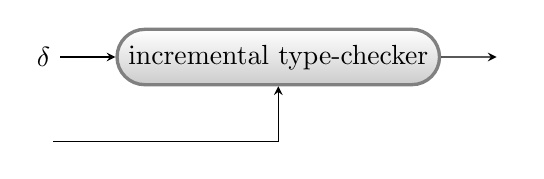
\begin{tikzpicture}[node distance=2em, >=stealth, hv
          path/.style={to path={-| (\tikztotarget)}}, vh
          path/.style={to path={|- (\tikztotarget)}} ]
          \node (term) {$\delta$}; \node (repo) [below=of
          term]{$\mr$}; \node[state] (tc) [right=of term] {incremental
            type-checker}; \node (repo2) [right=of tc] {$\mmr$};
          \path[->] (term) edge node {} (tc) (tc) edge node {} (repo2)
          (repo) edge [in=-90, out=0, hv path] node {} (tc) ;
        \end{tikzpicture}
      \end{figure}
    \end{block}
  \end{onlyenv}

  \begin{onlyenv}<3>
    \begin{block}{Instances of this problem}
      \begin{itemize}
      \item Separate type-checking (granularity = file)
      \item Version storage
      \item Module system
      \end{itemize}
    \end{block}
    \begin{block}{Challenges}
      Given a typed language:
      \begin{itemize}
      \item What language for deltas?
      \item What data structures for repositories?
      \item What \emph{commit} algorithm?
      \item What safety?
      \end{itemize}
    \end{block}
  \end{onlyenv}

\end{frame}

\begin{frame}{\textcolor{greenish}{Example}}
\end{frame}

\begin{frame}[fragile]{Memoization}
  \begin{overlayarea}{\textwidth}{14em}

    \begin{onlyenv}<1-2>
      \begin{lstlisting}
let check0 check env = function
  | Var x -> List.assoc x env
  | Lam (x, a, t) ->
    let b = check ((x, a) :: env) t in Arr (a, b)
  | App (t, u) -> match check env t with
      | Arr (a, b) when check env u = a -> b
      | _ -> failwith "wrong application"

let rec check env t = check0 check env t
      \end{lstlisting}
      \pause\vspace{1em}
      \begin{itemize}
      \item Builds the derivation on the stack
      \item Discards it
      \end{itemize}
    \end{onlyenv}

    \begin{onlyenv}<3-4>
      \begin{lstlisting}
module M = Map.Make(struct type t = env * tm
                        let compare = (=) end)

let tbl = ref (M.empty : tp M.t)

let rec check env t =
  try M.find (env, t) !tbl with Not_found ->
    let a = check0 check env t in
    tbl := M.add (env, t) a !tbl; a
      \end{lstlisting}
      \pause\pause\vspace{1em}
      \begin{itemize}
      \item Table $\mathsf{tbl}$ contains derivation
      \item If $\mathsf{tbl}(\Gamma, M) = A$ then $\Gamma\vdash M : A$
      \end{itemize}

    \end{onlyenv}

    \begin{onlyenv}<5>
      \begin{block}{Achievements}
        \begin{itemize}
        \item Detect syntactically equal (env, term)
        \item Reuse associated derivation
        \item Random access to sub-derivations
        \end{itemize}
      \end{block}
      \begin{block}{Limitations}
        \begin{itemize}
        \item Strictly syntactical reuse
        \item How can I trust the added code?
        \end{itemize}
      \end{block}
    \end{onlyenv}

  \end{overlayarea}
\end{frame}

\begin{frame}{A language for derivations}
  Let us take an off-the-shelf metalanguage: ELF.
  \begin{itemize}
  \item Signature $\Sigma$ = typing rules
  \item
  \end{itemize}
\end{frame}

\begin{frame}{}
  
\end{frame}
\subsection{Safe}

% mémoization? -> besoin d'un certificat

\section{Metalanguage}

\subsection{Requirements}

\subsection{}

\end{document}